\section{Durchführung}

Für diesen Versuch wird ein modular aufgebauter Verstärker verwendet. Dieser besteht
aus einem Vorverstärker, den Filtern, einen Phasenschieber, einem Funktionsgenerator,
einem Rauschgenerator, einem Tiefpass-Verstärker und einem Amplituden-/Lock-In-Detektor.
Dieser Verstärker ist in Abbildung (\ref{abb:2}) dargestellt.

\begin{figure}[H]
  \centering
  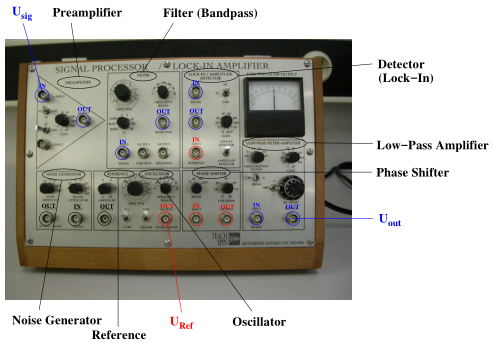
\includegraphics{Verstaerker.png}
  \caption{Darstellung des modular aufgebauten Verstärkers \cite{1}.}
  \label{abb:2}
\end{figure}

Als erstes soll der Funktionsgenerator untersucht werden. Dabei wird untersucht bei
welchem Ausgang die Spannungsamplitude verändert werden kann und bei welchem das nicht
möglich ist. Der Ausgang bei dem das nicht möglich ist, ist für das Referenzsignal.

Daraufhin soll die in Abbildung (\ref{abb:3}) gezeigte Schaltung gebaut werden. Der
Funktionsgenerator soll ein sinusförmiges Signal als Nutzsignal und ein sinusförmiges
Signal als Referenzsignal produzieren. Die resultirende Spannung wird erst ohne den
Tiefpass auf einem Oszilloskop dargestellt und danach mit dem Tiefpass.

\begin{figure}[H]
  \centering
  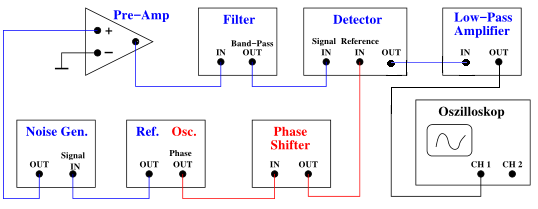
\includegraphics{Schaltung1.png}
  \caption{Schaltung des Lock-In-Verstärkers für den ersten Teil des Versuches \cite{1}.}
  \label{abb:3}
\end{figure}

Als nächstes wird mit dem Rauschgenerator ein Rauschsignal hinzugegeben. Für diesen
Fall wird wieder die resultirende Spannung erst ohne den Tiefpass dargestellt und
danach mit dem Tiefpass.

Zum Schluss wird die Intensität einer Leuchtdiode gemessen. Dazu wird die in Abbildung
(\ref{abb:4}) gezeigte Schaltung benötigt. Die Leuchtdiode soll mit einer Frequenz
von \SI{50}{\hertz} bis \SI{500}{\hertz} blinken und das Signal wird von einer Photodiode empfangen.
Nun wird die Intensität des Lichtes in gewissen Abständen gemessen.

\begin{figure}[H]
  \centering
  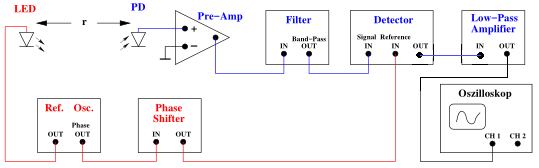
\includegraphics{Schaltung2.png}
  \caption{Schaltung des Lock-In-Verstärkers mit der Leuchtdiode \cite{1}.}
  \label{abb:4}
\end{figure}
